\chapter{Introduction}
\label{ch:intro}

Augmented Reality (AR) is technology that enables the seamless merging of the real world with virtual content (including visual and audio) so that both real and virtual can be seen and interacted with at the same time. Azuma defined AR as the coexistence of the virtual world and the real world, and that "it would appear to the user that the virtual and real objects coexisted in the same space"  \cite{azuma1997survey}. Milgram defined the mixed reality (MR) continuum (Figure \ref{fig:mr-continuum}) and placed AR between virtual reality (VR) where full immersion of virtual contents and augmented virtuality (AV) where mostly virtual content is overlaid by real content \cite{Milgram1995a}. 

% \begin{figure}
%     \centering
%     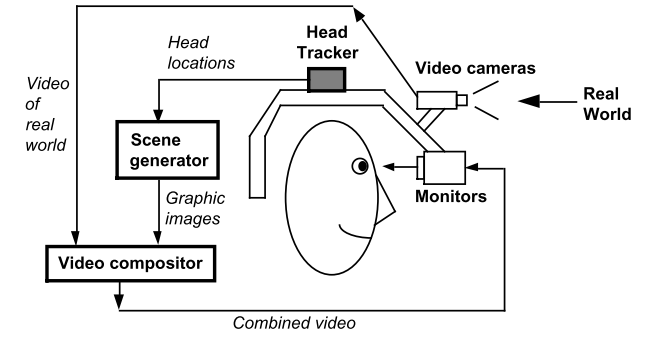
\includegraphics[width=.8\linewidth]{images/video-see-through-ar.png}
%     \caption{A video see-through AR display}
%     \label{fig:video-see-through}
% \end{figure}

\begin{figure}
    \centering
    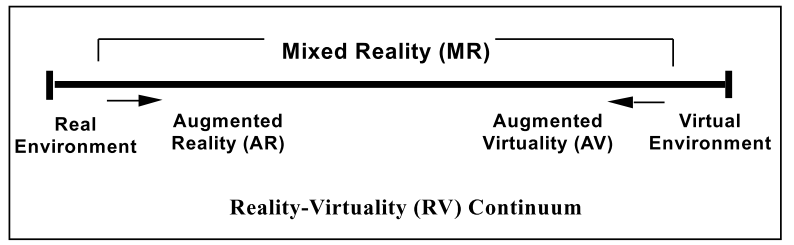
\includegraphics[width=.8\linewidth]{images/mixed-reality-continuum.png}
    \caption{The mixed reality continuum by Milgram \cite{Milgram1995a}}
    \label{fig:mr-continuum}
\end{figure}

Social interactions are important because...\todo[inline]{importance}

The needs and reasons for using AR for social interactions are... \todo[inline]{needs}

AR could improve social interactions by... \todo[inline]{improvement expected}


In \cite{Zhou2008} and \cite{Kim2018} looked at trends in AR in the academic conference ISMAR\footnote{http://www.ismar.net/} and in the research community as a whole, and reported "\textit{AR technology will continue to develop even more dynamically and effectively over the next ten years, toward the vision of pervasive presence in our daily lives.}" \cite{Kim2018}. AR displays are getting more affordable with better rendering and registration techniques. Also, AR displays are becoming more self-contained and lighter which enables mobile AR applications.

In a review about the historic uses of wearable displays and AR displays \cite{Peddie2017}, it started in 1940 with the first heads-up display (HUD) in the UK. Then in the 1960s, most uses of AR were to build AR helmet for pilots field of view. Then interest in AR started increasing in 2009 when Lego introduced AR Digital box, then started relative decline since Google Glass was introduced in 2012. In the Gartner 2019 trends report \cite{gartner2019}, it shows that AR and immersive technologies have been getting out the disillusionment phase of the hype cycle and moving toward a steady adoption and day to day scenarios in the next 5-10 years.

Social interactions have been studied in the past. 
\cite{AlanKellerGomes} looked into...

\cite{Damian2015}
\cite{Wilson2012a} reviews Facebook social interactions 

\section{Problem Statement}

The focus of this thesis is on enabling the use of wearable AR for sharing social experiences. The gap between the vision of social AR and the current state of the art is... \todo[inline]{gap..}

This PhD thesis addresses the problems of: 

\begin{enumerate}
    \item using visualising and interacting with social contacts through wearable AR displays.
    \item displaying a large amount of 3D content of sharing social data that is overlaid over a limited available physical space through wearable AR devices.
    \item defining and exploring the best ways to use wearable AR devices to connect with social networks.
\end{enumerate}

Previously, handheld AR systems have been used to view social networks in a number of different ways. For example, Presslite's Twitter 360\footnote{https://www.youtube.com/watch?v=5w7EAz8-uwU} (Figure \ref{fig:presslite}) shows virtual tweets overlaid on the real world at the locations of the people that sent them , and early versions of Junaio\footnote{https://en.wikipedia.org/wiki/Junaio} allowed people to drop virtual messages and pictures in the real world, as did the popular application Sekai Camera\footnote{https://www.youtube.com/watch?v=oxnKOQkWwF8}. Most of these applications were focused on asynchronous collaboration, enabling people to post virtual messages in space which can later be browsed and retrieved by other users. 

\begin{figure}
    \centering
    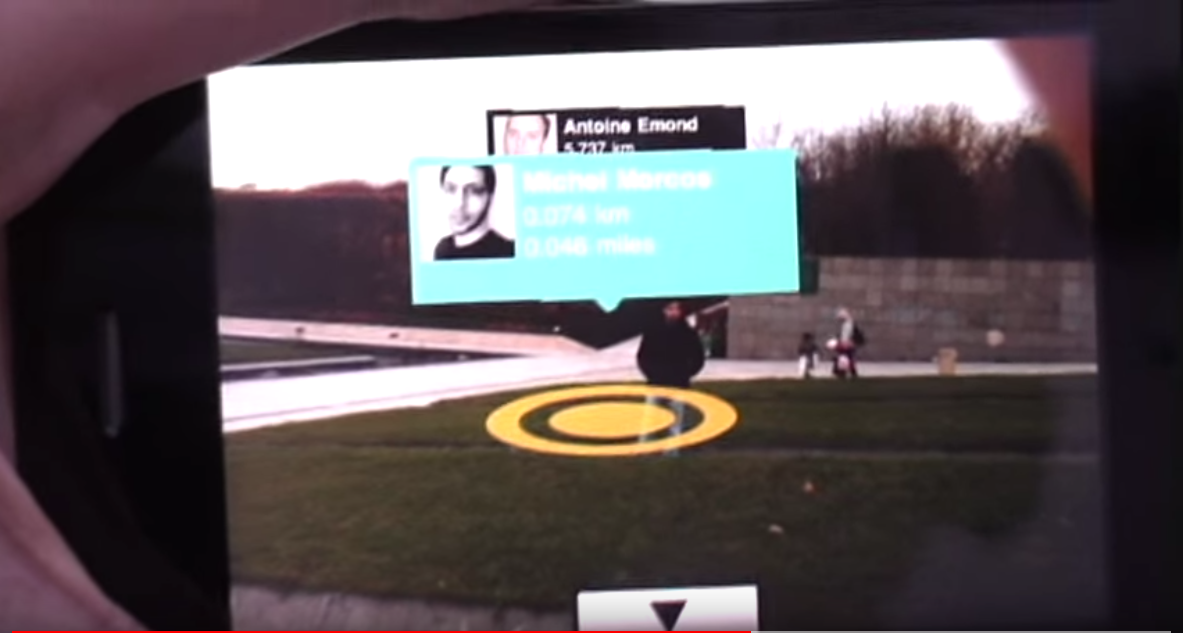
\includegraphics[width=.8\linewidth]{images/Presslite-twitter-360.PNG}
    \caption{Presslite's Twitter 360 AR interface by Twitter in 2009}
    \label{fig:presslite}
\end{figure}

However, similar technology could also be used for live synchronous collaboration such as live video avatar sharing~\cite{Billinghurst2002}, sharing realistic 3D models superimposed over the real world~\cite{Fanello2016}, or by using virtual avatars to show a live view of remote collaborators and their surrounding space as in the Holoportation system~\cite{Fanello2016} (Figure \ref{fig:holoportation}).

\begin{figure}
    \centering
    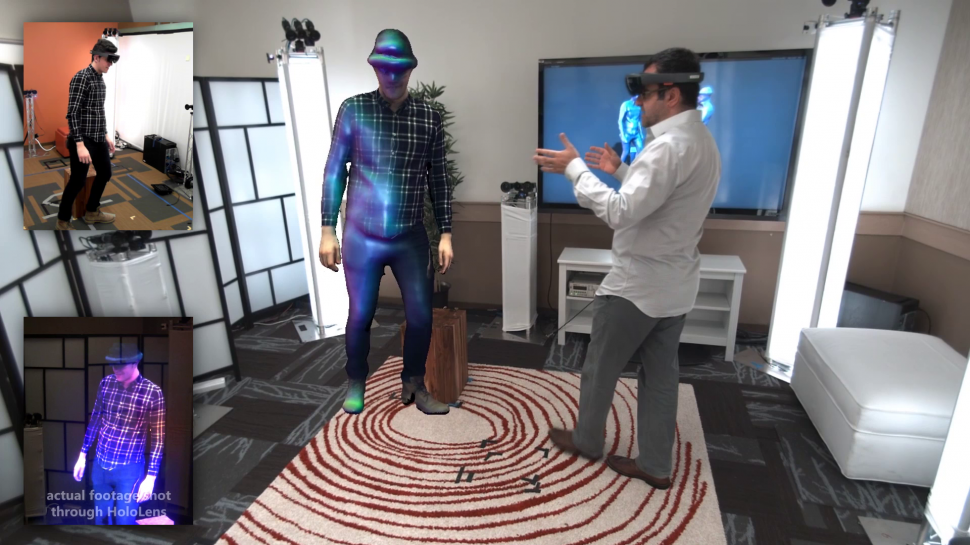
\includegraphics[width=.8\linewidth]{images/holoportation.png}
    \caption{Holoportation by Microsoft \cite{Fanello2016}}
    \label{fig:holoportation}
\end{figure}

% - The potential for AR to be a social sharing platform. \\
% - Sharing social experiences was not fully addressed in the research community

With major industry players (e.g., Microsoft, Facebook and Magic Leap) supporting AR, a potential use of AR could be for connecting with social networks. Just as people today use their mobile phones to connect with hundreds or thousands of friends, wearable AR displays could be used to connect with friends and view and interact with their shared information.

Applications for Social VR and 360-degree video have been introduced on new VR headsets. For instance, Facebook Spaces\footnote{https://www.facebook.com/spaces} allows VR users to connect with friends and family and share 360-degree photos and take selfies. AltSpaceVR\footnote{https://altvr.com/} was acquired by Microsoft and enables more diverse hand-held and wearable devices to be used for social connection with others. Most recently, Magic Leap's Avatar Chat\footnote{https://www.magicleap.com/stories/blog/connect-with-friends-with-avatar-chat}(Figure \ref{fig:ml-avatar-chat}) offers similar experiences where avatars representing social friends are displayed in an AR space . 


\begin{figure}
    \centering
    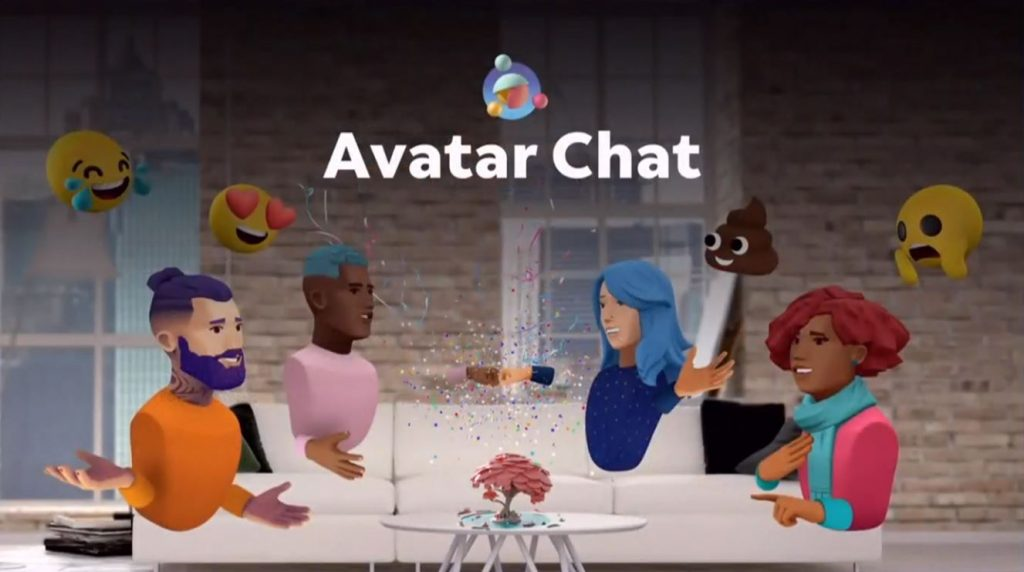
\includegraphics[width=.8\linewidth]{images/magic-leap-avatar-chat.jpg}
    \caption{Magic Leap's Avatar Chat by Magic Leap in 2018}
    \label{fig:ml-avatar-chat}
\end{figure}

By using a wearable AR display like the Microsoft HoloLens\footnote{https://www.microsoft.com/en-nz/hololens}, it could be possible for the user to see an AR representation of their social network visible at all times. However, this raises the question of how to visually represent the user's contacts in the network. For example, if a user has a large social network with hundreds of contacts available, visually representing each of them might clutter the user's visual space.

\section{Research Questions}

This thesis targets the future where AR devices are used every day, and social networks are visualised in the AR view. The overarching research question is \textit{how AR can be be used for sharing social experiences in both remote and face to face social contacts}. We address the following research questions: 

\begin{enumerate}[label=RQ\arabic*]
    % (chapter 3 - Social AR continuum)
    \item{\label{rq:continuum}What dimensions/factors/parameters in sharing social experiences on wearable AR devices?
    % \\(option 1): How to represent social networks and shared social data on wearable AR devices?
    % \\(option 2): What dimensions/factors/parameters in sharing social experiences on wearable AR devices?
    }
    % (chapter 4 - annotation continuum)
    \item{\label{rq:interaction}How wearable AR displays can be used best for interacting with social contacts and shared social data?
    % \\(option 1): How to represent annotations/tags on wearable AR devices for shared social experiences?
    % \\(option 2): How annotations/tags are used as interaction method in social AR? 
    % \\(option 3): What are the options/parameters of annotation that can be changed in social AR?
    }
    % (chapter 5 - Sharing data continuum)
    \item{\label{rq:data}What is the best way of to view and interact with shared social data on AR displays?
    % \\(option 1): How to share virtual objects/data with our social network on wearable AR devices?
    % \\(option 2): What are the options of sharing social data in AR?
    % \\(option 3): How sharing data is placed on the social AR continuum?
    }
    % (chapter 6 - visualising social contacts) 
    \item{\label{rq:people}What dimensions work best for visualising and interacting with social contacts through wearable AR displays?
    % \\(option 1): How to visualise our social contacts as virtual avatars on wearable AR devices?
    % \\(option 2): What are the options of visualising contacts on social AR?
    % \\(option 3): How visualising social contacts is placed on the social AR continuum?
    % \\(option 4): What is the impact of visualising social contacts on social presence?
    % \\(option 5): What is the impact on social presence of different visualisation methods for social contacts?
    }
\end{enumerate}

To answer the research questions, this thesis explores how wearable AR can be used for sharing social experiences. These explorations identify the parameters through which AR sharing for social reasons happen. Once the parameters are defined, we build a system prototypes as a proofs of concept of the experiences or interaction designs. We then run user studies to test the objectives of each system with human participants. We observe their behaviour and report on the results of these experiments. 

Chapter \ref{ch:continuum}: "The Social AR Continuum" aims to answer \ref{rq:continuum} with describing the overall dimensions on the social AR continuum. Chapter \ref{ch:annotation} "Annotation Continuum" aims to answer \ref{rq:interaction} with exploring annotations and tags for sharing social experience. Chapter \ref{ch:data} "Sharing Data Continuum" focuses more about the data being shared with social contacts and aiming to answer \ref{rq:data}. Chapter \ref{ch:contacts} "Visualising Social Contacts" aims to answer \ref{rq:people} by exploring visualising social contacts. 

\section{Contributions}

The following summarises the contributions of this thesis: 

\begin{enumerate}
    \item We identify the parameters and dimensions of the social AR continuum. The main contribution is defining the social AR continuum which consists of a set of parameters that define the space of sharing social experiences through wearable/hand-held AR devices. We define the space of the AR continuum by exploring the main parameters that can be varied based on social proximity. These parameters are grouped into the following categories 1) self and other, 2) shared objects and annotation and 3) surrounding environment. Under each of these categories, we define the dimensions of variables that affect the shared social experience.
    
    \item We implemented several social AR experiences in terms of user interfaces. For each dimension defined on the continuum, we built software prototypes to test the user interface design with human subjects. The implementation details are described in the thesis for future use.
    
    \item We conducted user studies to evaluate and validate the parameters of the social AR continuum. Using the prototypes we constructed, a series of user-studies and focus-groups were conducted to validate the dimensions of the social AR continuum.
    
    \item We synthesised high-level design guidelines for interface designers looking to build social sharing experiences on AR devices. One of the outcomes of defining the social AR continuum and validating these dimensions is that our work can serve as high-level experience design guidelines that help individuals and organisations to create effective AR experiences for social sharing and connection purposes.
\end{enumerate}

In summary, this thesis helps to increase the understanding of how to share social experiences through AR devices. The results of the user experiments conducted throughout this research help identify the impact of the social AR continuum parameters on presence, user engagement and user interface usability, which serves as guidelines for future designs. 

The rest of the thesis is organised as follows: Chapter \ref{ch:continuum} describes the social AR continuum and the parameters/dimensions involved. Chapter \ref{ch:annotation} describes the shared data and annotation continuum including different implementations of shared annotation and awareness cues on different platforms (hand-held and wearable). Chapter \ref{ch:data} describes the surrounding environment continuum including shared 360-degree videos and 30 captured spaces. Chapter \ref{ch:contacts} describes the continuum of self and others of representing social contact networks on AR devices. The following diagram (Figure \ref{fig:thesis-outline}) shows the structure of the thesis and how it answers the research questions. 

\begin{figure}
    \centering
    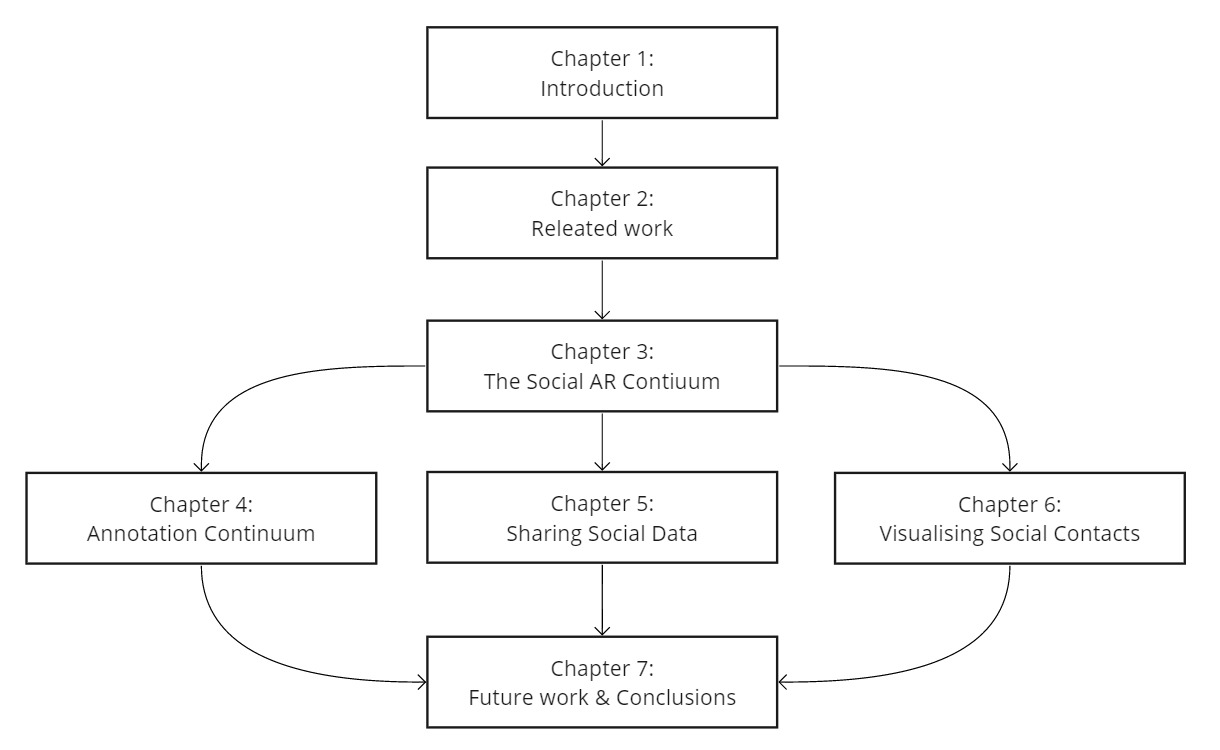
\includegraphics[width=\linewidth]{images/thesis-outline.png}
    \caption{Thesis outline}
    \label{fig:thesis-outline}
\end{figure}

\section{Selected Publications}

Most of the work of this thesis has been submitted, peer-reviewed and published at scientific conferences and journals specialising in the AR, HCI and computer graphics fields. This list contains selected publications that are relevant to this thesis. 

The following publication defines the concept of the social AR continuum and describes a focus group and a user study implementing visualising social contacts through AR headset, and addressing RQ1. 

\begin{itemize}
    \item{ \fullcite{Nassani2017a}}
\end{itemize}

The following publications focus on placing AR annotations/tags on shared 360-degree panoramas and video streaming content, addressing RQ2.

\begin{itemize}
    \item{ \fullcite{Nassani2016}}
    \item{ \fullcite{Nassani2015}}
    \item{ \fullcite{Nassani2015a}}    
    \item{ \fullcite{Reichherzer2014}}
    \item{ \fullcite{Billinghurst2014}}
\end{itemize}

The following publications focus on shared surrounding environments and changing the levels of detail based on social proximity, addressing RQ3.

\begin{itemize}
    \item{ \fullcite{Nassani2018a}}
    \item{ \fullcite{Nassani2018b}}
    % \item{ \fullcite{Nassani2018c}} -- frontier paper rejected
\end{itemize}

The following publications focus on visualising social contacts based on social proximity, addressing RQ4. 

\begin{itemize}
    \item{ \fullcite{Nassani2017b}}
    \item{ \fullcite{Nassani2017}}
\end{itemize}

The above publications help to answer the research questions of this thesis, including how to share social experiences on AR devices for each category on the social AR continuum. 


% \todo[inline]{Mark: In the remainder of the thesis we first review related work and explain the research gap that our work files (section 2). Then [put  more here – summarise the thesis structure] }

% \todo[inline]{[You may also want to put together a  thesis outline chart. Basically showing the experiments you conducted and  prototypes you developed and  how these  contribute to addressing  the research questions that you’ve raised. This is helpful if you have a lot of material to report on, so the reviewers can understand how it all fits together] }